\documentclass{beamer}[10]
\usepackage{pgf}
\usepackage[danish]{babel}
%\usepackage[english]{babel}
\usepackage[utf8]{inputenc}
\usepackage{beamerthemesplit}
\usepackage{graphics,epsfig, subfigure}
\usepackage{url}
\usepackage{srcltx}
\usepackage{hyperref}
\usepackage[style=ieee]{biblatex}
\usepackage{graphicx}
\usepackage{bm}
\addbibresource{biblatex-examples.bib}

%package for the copyright symbol
\usepackage{textcomp}

%you can repeat this command to define different colors here.
\definecolor{kublue}{RGB}{86,160,209}

\setbeamercovered{transparent}
\mode<presentation>
\usetheme[numbers,totalnumber,compress,sidebarshades]{PaloAlto}
%\setbeamertemplate{footline}[frame number]
\setbeamertemplate{footline}[text line]{%
  \parbox{\linewidth}{\vspace*{-8pt}
  						%Copyright \textcopyright 2015 by Milind A. Phadnis. All rights reserved. \hfill
  						%\insertshortauthor\hfill
  						%\insertpagenumber}
}}

  \usecolortheme[named=kublue]{structure}
  \useinnertheme{circles}
  \usefonttheme[onlymath]{serif}
  \setbeamercovered{transparent}
  \setbeamertemplate{blocks}[rounded][shadow=true]

\logo{
\includegraphics[width=1.5cm]{KU-Med-Logo.jpg}}
%\useoutertheme{infolines} 
\title{A Safety Signal Analysis with Three-Level Hierarchical Mixture Model}
\author{Guanlin Zhang}
\institute{Department of Biostatsitics \\ University of Kansas Medical Center}
\date{27 Nov 2018}



\begin{document}
\frame{\titlepage \vspace{-0.5cm}
}

%\frame
%{
%\frametitle{Overview}
%\tableofcontents%[pausesection]
%}

%Introduction corresponding to the introduction section of manuscript
\section{Introduction}

\begin{frame}
	\frametitle{Introduction}
	\begin{block}{Some background}
		\begin{enumerate}
			\item trials with treatment and control group (two arms);
			\item want to understand if treatment (or drug) cause adverse effects;
			\item we have many adverse effects categorized under different body systems.
		\end{enumerate}
	\end{block}
\end{frame}
\begin{frame}
	\frametitle{Introduction}
	\begin{figure}
		\centering
		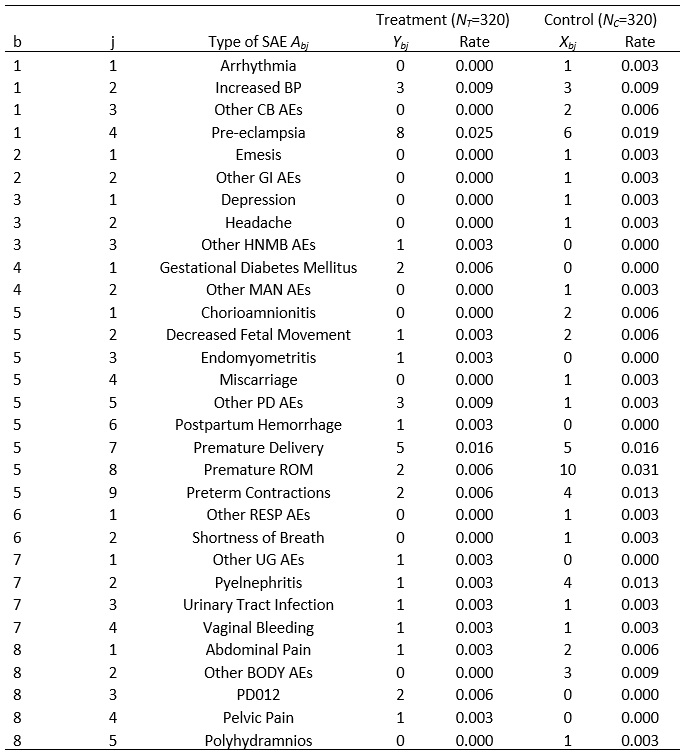
\includegraphics[width = 6cm]{data.jpg}
		\caption{data example}
	\end{figure}
\end{frame}

\section{Model}

\begin{frame}
	\frametitle{Model}
	We follow the three-level hierarchical model proposed in [\cite{Berry04}]
	\begin{center}
		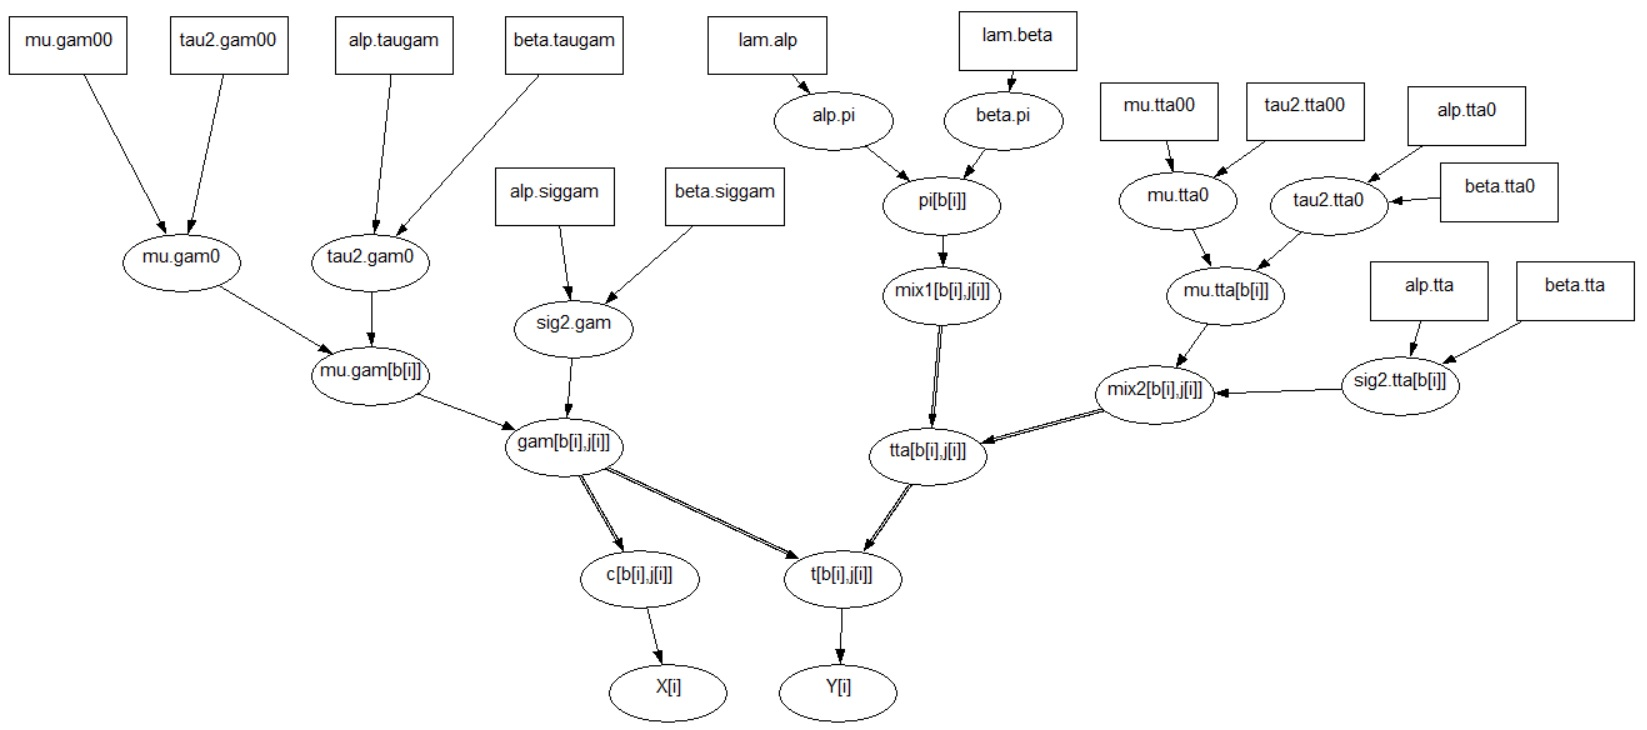
\includegraphics[width = 10cm]{doodle.jpg}
	\end{center}
\end{frame}

\begin{frame}
	\frametitle{Goal}
	We have the following goals:
	\begin{block}{ }
		\begin{enumerate}
			\item Fit the original data from [\cite{Berry04}](OpenBUGS and R) and compare
			\item Fit the hierarchical model to the example data and compute posterior probabilities (OpenBUGS and R)
			\item Fit another independent model to the example data and compare results with hierarchical model
		\end{enumerate}
	\end{block}
\end{frame}

\section{Results}
\begin{frame}
	\frametitle{OpenBUGS vs R vs Original Results}
	The following table compares results on the original data in [\cite{Berry04}]:
	\begin{table}[ht]
  \centering
  \tiny
  \begin{tabular}{|l|c|c|c|c|c|}
  \hline
  \cline{1-2}\cline{3-5}
  \multicolumn{2}{|c|}{}& \multicolumn{3}{|c|}{post $P(\theta > 0)$} & \\
    \hline
  AEs& Type & Reference & OpenBugs & R & Fisher exact p\\
    \hline
    Irritability & $\theta_{8, 3}$ & $0.78$ & $0.978$ & $0.984$ & 0.003\\
    Diarrhea &  $\theta_{3, 4}$ & $0.231$ & $0.847$ & $0.853$  & 0.029\\
    Rash & $\theta_{10, 4}$ & $0.19$ & $0.945$ & $0.993$ & 0.021\\
    Rash, measles/rub-like & $\theta_{10, 6}$ & $0.126$ & $0.890$ & $0.946$ & 0.039\\
  \hline
  \end{tabular}
  \caption{OpenBugs and R results compare with reference}\label{tab:berry_compare}
\end{table}
\end{frame}

\begin{frame}
	\frametitle{Independent Model}
	We compare hierarchical model with independent model when fitting the example data:
	\begin{center}
		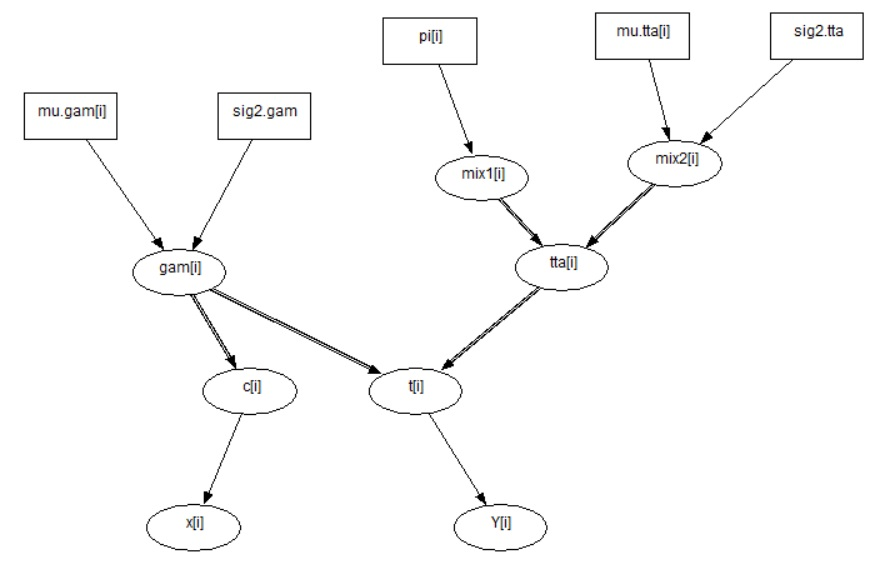
\includegraphics[width = 10cm]{doodle_ind.jpg}
	\end{center}
\end{frame}

\begin{frame}
	\frametitle{Results}
	\begin{figure}
	\tiny
	\centering
		\includegraphics[width = 8cm]{results.jpg}
	\end{figure}
%	\begin{table}
%	\centering
%	\tiny
%\begin{tabular}{|l|c|c|c|}
%  \hline
%  \cline{2-4}
%  \multicolumn{1}{c}{} & \multicolumn{3}{|c|}{post $P(\theta > 0)$}\\
%  \hline
%  AE & R(Hierarchical)& OpenBUGS(Hierarchical)& OpenBUGS(Independent)\\
%  \hline
%  Arrhythmia &$0.0207$& $0.0267$ & $0.0496$\\
%  Increased BP&$0.0487$& $0.0591$ & $0.0939$\\
%  Other CB AEs &$0.0136$& $0.0237$ & $0.0227$\\
%  Pre-eclampsia &$0.0763$& $0.1102$ & $0.1058$\\
%  \hline
%  Emesis&$0.0258$& $0.0264$ & $0.0457$\\
%  Other GI AEs&$0.022$& $0.0249$ & $0.0463$\\
%  \hline
%  Depression&$0.0229$& $0.0275$ & $0.0464$\\
%  Headache &$0.0232$& $0.0301$& $0.0508$\\
%  Other HNMB AEs&$0.046$& $0.0529$ & $0.2012$\\
%  \hline
%  Gestational Diabetes Mellitus &$0.0763$& $0.0961$ & $0.2920$\\
%  Other MAN AEs&$0.0331$& $0.0341$ & $0.0476$\\
%  \hline
%  Chorioamnionitis&$0.0061$& $0.0156$ & $0.0240$\\
%  Decreased Fetal Movement &$0.0199$& $0.0281$ & $0.0661$\\
%  Endomyometritis &$0.037$& $0.0413$& $0.1984$\\
%  Miscarriage &$0.0062$& $0.0194$ & $0.0493$\\
%  Other PD AEs &$0.0634$& $0.0718$ & $0.2238$\\
%  Postpartum Hemorrhage &$0.0309$& $0.0406$ & $0.1871$\\
%  Premature Delivery &$0.0486$& $0.0671$ & $0.0708$\\
%  Premature ROM &$0.0059$& $0.0109$ & $0.0045$\\
%  Preterm Contractions &$0.0186$& $0.0331$ & $0.0434$\\
%  \hline
%  Other RESP AEs &$0.0113$& $0.0232$ & $0.0472$\\
%  Shortness of Breath &$0.0105$& $0.0251$ & $0.0474$\\
%  \hline
%  Other UG AEs &$0.0466$& $0.0508$ & $0.1887$\\
%  Pyelnephritis &$0.0254$& $0.0313$ & $0.0272$\\
%  Urinary Tract Infection &$0.0466$& $0.0452$ & $0.1047$\\
%  Vaginal Bleeding &$0.0402$& $0.0473$ & $0.1046$\\
%  \hline
%  Abdominal Pain &$0.0335$& $0.0434$ & $0.0616$\\
%  Other BODY AEs &$0.0125$& $0.0213$ & $0.0118$\\
%  PD012 &$0.0502$& $0.074$ & $0.2885$\\
%  Pelvic Pain &$0.0414$& $0.0542$ & $0.1897$\\
%  Polyhydramnios& $0.0198$& $0.0268$& $0.0483$\\
%  \hline
%\end{tabular}
%  \caption{hierarchical model vs independent model, and winBUGS vs R}\label{tab:newcompare}
%\end{table}
\end{frame}

\appendix
\section<presentation>*{References}

\begin{frame}[allowframebreaks]
  \frametitle<presentation>{References}
    
\begin{thebibliography}{10}
%    
 \beamertemplatebookbibitems
 
 \bibitem{Berry04}Berry, Scott M. and Berry, Donald A. (2004). Accounting for Multiplicities in Assessing Drug Safety: A Three-Level Hierarchical Mixture Model. \emph{Biometrics}{\bf 60}, 418-426

%\bibitem{Allison10}Allison, Paul D. (2010) \emph{Survival Analysis Using SAS: A Practical Guide, 2nd Edition}. SAS Institute Inc., Cary, NC, USA.
%
%\bibitem{Cap94}Caplan, R.J., Pajak, T.F. and Cox, J.D. (1994). Analysis of probability and risk of cause-specific failure. \emph{International Journal of Radiation Oncology.} \emph{Biology, Physics.} {\bf 29}, 1183-1186.
%
%\bibitem{Cox84}Cox, D.R. and Oakes, D.(1984) \emph{Analysis of Survival Data.} London: Chapman$\&$ Hall.
%
%\bibitem{Fine99}Fine, Jason P., and Gray, Robert J., (1999) A proportional Hazards Model for the Subdistribution of a Competing Risk. \emph{Journal of the American Statistical Association} Vol. 94, No. 446,  496-509.
%
%\bibitem{Gel90} Gelman, R., Gelber, R., Henderson, I.C., Coleman, C.N. and Harris, J.R.(1990). Improved methodology for analyzing local and distant recurrence. \emph{Journal of Clinical Oncology}. {\bf 8}, 548-555.
%
%\bibitem{Goo99} T. A., Leisenring, W., Crowley, J. and Storer, B. E. (1999). Estimation of failure probabilities in the presence of competing risks: new representations of old estimators. \emph{Statistics in Medicine, }{\bf 18}, 695-706.
%
%\bibitem{Kalb02} Kalbfleisch, J.D. and Prentice, R.L. \emph{The Statistical Analysis of Failure Time Data.} Hoboken, NJ: John Wiley $\&$ Sons, Inc.
%
%\bibitem{Klein97} Klein, John P. and Moeschberger, Melvin L . \emph{Survival Analysis Techniques for Censored and Truncated Data} Springer. 1997.
%
%\bibitem{Peterson04} P.M., Gospodarowicz, M., Tsang, R., Pintilie, M., Wells, W., Hodgson, D., Sun, A., Crump, M., Patterson, B. and Bailey, D. (2004). Long-term outcome in stage I and II follicular lymphoma following treatment with involved field radiation therapy alone. \emph{Journal of Clinical Oncology}, {\bf 22}, 563S.
%
%\bibitem{pintilie06} Pintilie, Melania. \emph{Competing Risks: A practical Perspective} John Wiley $\&$ Sons, Ltd. 2006.
%
%\bibitem{Scheike08}Scheike, T.H., Zhang, M., and Gerds, T.A., Predicting Cumulative Incidence Probability by Direct Binomial Regression, \emph{Biometrika}, {\bf 95}, 205-220.

%\bibitem{aans}http://www.aans.org/Patients/Neurosurgical-Conditions-and-Treatments/Concussion
%
%\bibitem{agresti} Agresti, A. \newblock{ Categorical Data Analysis.} John Wiley \& Sons, Inc.  3rd Edition,  2013.
%
%\bibitem{barnes} Barnes BC, Cooper L, Kirkendall DT, McDermott TP, Jordan BD, Garrett WE Jr. \newblock{Concussion history in elite male and female soccer players.} Am J Sports Med. 1998;26:433-438.
%
%\bibitem{biausa} http://www.biausa.org/concussion/whatisaconcussion
%
%\bibitem{boden} Boden BP, Kirkendall DT, Garrett WE Jr. \newblock{Concussion incidence in elite college soccer players.} Am J Sports Med. 1998;26:238-241.
%
%\bibitem{collins} Michael W. Collins, Anthony P. Kontons, David O.Okonkwo, et al. \newblock{Concussion is Treatable: Statements of Agreements from the Targeted Evaluation and Active Management(TEAM) Approaches to Treating Concussion Meeting held in Pittsburg, October 15-16, 2015.} Neurosurgery. 2016 Dec; 79(6): 912-929.
%
%\bibitem{eva} Evans R W. \newblock{The postconcussion syndrome: 130 years of controversy.} Semin Neurol. 1994; 14:32-39.
%
%\bibitem{gro} Gronwell DMA, Wringtson, P. \newblock{Cumulative effect of concussion.} Lancet. 1975; 2: 99-997
%
%\bibitem{iss}   National Collegiate Athletic Association..  \newblock{NCAA Injury Surveillance System for Academic Years 1997–2000.}  Indianapolis, IN: National Collegiate Athletic Association; 2000..  
%
%\bibitem{lang} Langois JA, Rutland-Brown W, Wald MM. \newblock{The epidemiology and impact of traumatic brain injury: a brief overview.} J Head Trauma Rehabil. 2006;21:375-378.
%
%\bibitem{main}   Covassin T.,   Swanik C. B.,  and M. L. Sachs.  \newblock{Sex Differences and the Incidence of
%Concussions Among Collegiate Athletes}, Journal of Athletic Training,  38(3): 238-244, 2003.  
%  
%%  \bibitem{Kac56}
%%Mark Kac
%%\newblock{Some stochastic problems in physics and mathematics}. Magnolia Petroleum Co. Colloq. Lect. 2.
%
%%\bibitem{Goldstein51}
%%Goldstein
%%\newblock{On diffusion by discontinuous movements, and on the telegraph equation}. Quart. J. Mech. Appl. math. 4, 129-156.
%
 \end{thebibliography}
\end{frame}
%
\begin{frame}
	\frametitle{Thank You!}
	\begin{center}
		\includegraphics[width = 10cm]{thank-you.jpg}
	\end{center}
\end{frame}
%
%%\section{First section}
%%
%%\frame{
%%\frametitle{Sample Frame Title No. 1}
%%Try some English Lorem ipsum dolor sit amet, consectetur adipiscing elit, sed do eiusmod tempor incididunt ut labore et dolore magna aliqua. Ut enim ad minim veniam, quis nostrud exercitation ullamco laboris nisi ut aliquip ex ea commodo consequat. Duis aute irure dolor in reprehenderit in voluptate velit esse cillum dolore eu fugiat nulla pariatur. Excepteur sint occaecat cupidatat non proident, sunt in culpa qui officia deserunt mollit anim id est laborum.
%%}
%%
%%\subsection{Sample subsection}
%%
%%\frame{
%%\frametitle{Sample Frame Title No. 2}
%%\begin{itemize}
%%\item First item
%%\item Second item
%%\item Third item
%%\end{itemize}
%%}
%%
%%\section{Second section}
%%
%%\frame{
%%\frametitle{Sample Frame Title No. 3}
%%Lorem ipsum dolor sit amet, consectetur adipiscing elit, sed do eiusmod tempor incididunt ut labore et dolore magna aliqua. 
%%\begin{block}{Something important}
%%Einstein's formula
%%$$E=mc^2$$
%%\end{block}
%%}


\end{document}
